\section{Topic Dynamics of Tweets and News}
\label{sec:top}

In this part, we compare topic dynamics of news and tweets based on the results by \stlda. Considering the factor of distance on perception of events~\cite{he2015uncovering}, we analyze topic dynamics for tweets in and out of \stlouis where the Ferguson unrest took place to exclude the influence of geographical difference. To answer the research questions, we compare topics in news and tweets, and how the topic proportion changes everyday. First we related topic dynamics to ground truth events to see the different focus of media and the public, and how news and social media react to real situations. Then we compare topic dynamics of news and tweets in and out of \stlouis area to find out whether there is evidence of influence by media on the public, or shift focus of the media because of topics in tweets.

\begin{figure*}[htpb]
\centering
\subfigure[Tweets in \stlouis]
{
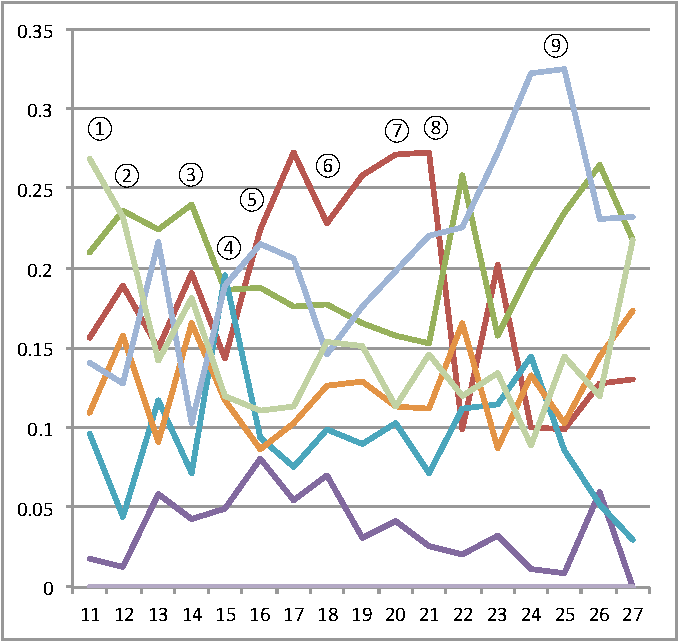
\includegraphics[width=0.32\linewidth]{figures/3LDA2TweetsInSt_revised.pdf}
\label{fig:tweets_topics_inst}
}
\subfigure[Tweets out of \stlouis]
{
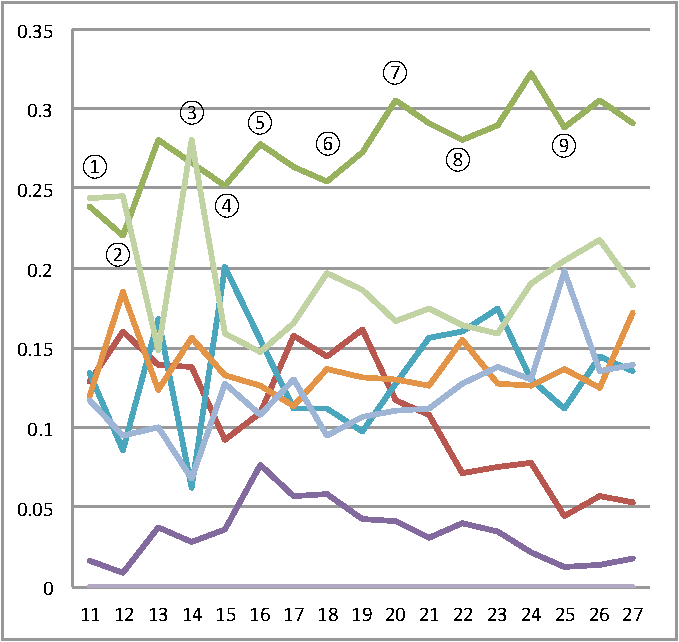
\includegraphics[width=0.32\linewidth]{figures/3LDA2TweetsOutSt_revised.pdf}
\label{fig:tweets_topics_outst}
}
\subfigure[News]
{
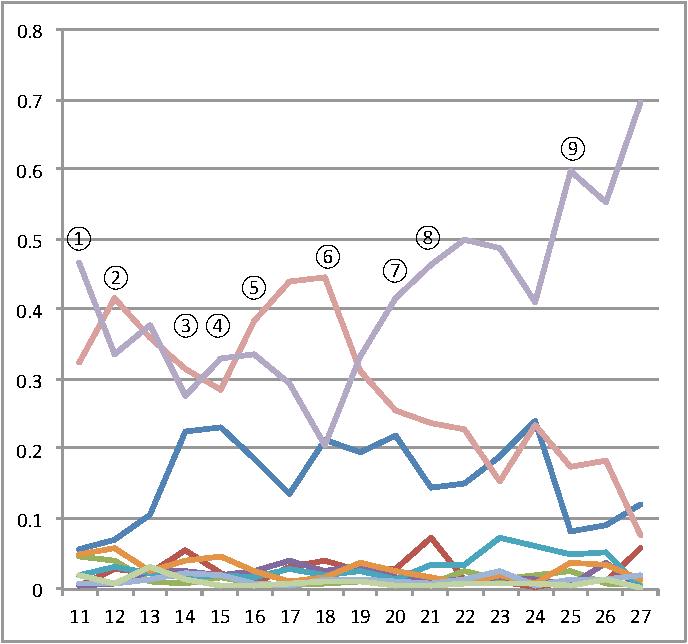
\includegraphics[width=0.32\linewidth]{figures/1STLDANews-2_revised.pdf}
\label{fig:news_topics}
}

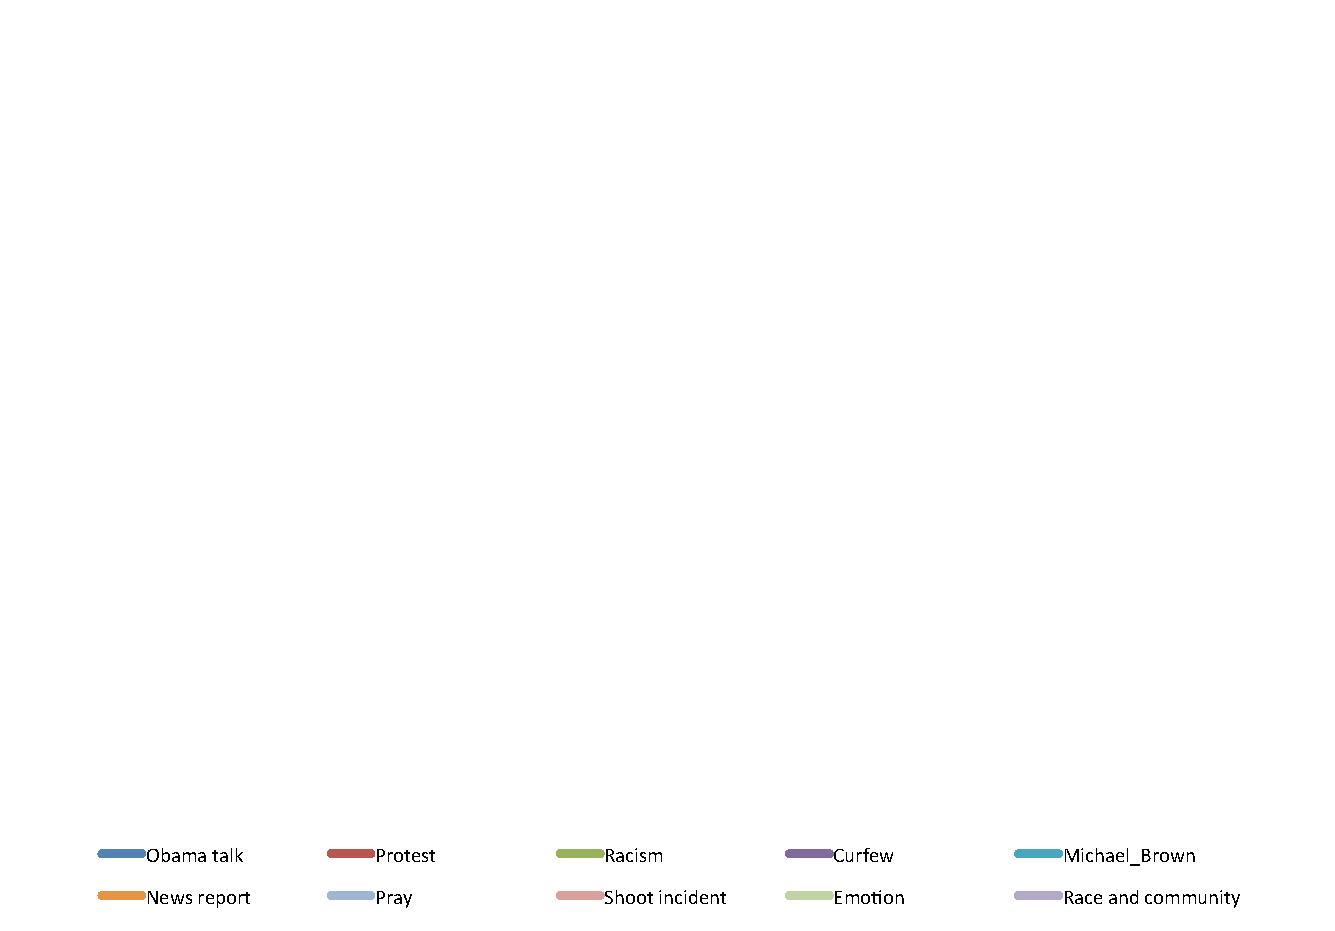
\includegraphics[width=\linewidth]{figures/Legend_revised_cut.pdf}
\caption{Topic Dynamics of Tweets and News by \stlda. Important events: \textcircled{\small{1}} Aug 11: unrest continues; \textcircled{\small{2}} Aug 12: first Obama talk; \textcircled{\small{3}} Aug 14: second Obama talk and Nixon announces law enforcement operation; \textcircled{\small{4}} Aug 15: robbery video is released; \textcircled{\small{5}} Aug 16: curfew is imposed; \textcircled{\small{6}} Aug 18: National Guard is deployed; \textcircled{\small{7}} Aug 20: a grand jury convenes to begin determining of crime and streets become quiet; \textcircled{\small{8}} Aug 21: National Guard withdrew; \textcircled{\small{9}} Aug 25: Michael Brown's funeral.}\label{fig:topic_dynamics}
\end{figure*}

\subsection{Focus Shift Analysis for Tweets and News}
\label{subsec:tweet_topic}
We relate topics of tweets discovered by \stlda with ground truth to analyze focus of the people and how the focus changes along with important events. Ground truth events and the import time points perform as benchmarks. We choose a news report that involves with timeline of important events since Michael Brown's death. Although it is from the view of the media, which have perspectives and may not include all important events, it is a relative complete benchmark with time of shoot incident, looting, FBI investigation, Obama talk, protests, curfew, Michael Brown's funeral and so on.\footnote{\url{http://www.telegraph.co.uk}}

\subsubsection{Tweet Topics in and out of \stlouis Area}
The tweet topic dynamics in and out of \stlouis are shown in Figure~\ref{fig:topic_dynamics}.

Difference in topic dynamics of two sets of tweets show different perception of events for people in and out of \stlouis area. More tweets in \stlouis talk about \protest, while out of \stlouis more tweets talk about \racism. From August 18, when Governor Nixon deployed the National Guard to Ferguson, to August 21 when the National Guard withdrew, protests and conflicts keep occurring. People in Ferguson area are closer and more related to protests, so tweets with this topic surge to take more than 25\% of all tweets. Meanwhile proportion of \protest tweets out of \stlouis is far less. The public not involved in the event tend to have less knowledge about real situations, but according to what they hear and know, they are better at abstract thinking, thus \racism takes majority in most of the time.

An interesting phenomenon is the \emotion topic change. Michael Brown was killed on August 9, and anger emotion is the major topic of tweets in \stlouis, then \emotion tweets keep decreasing, taking 10\% to 15\% of all tweets. However outside \stlouis area, there is a lag effect of \emotion explosion on August 14th. It is possible that news takes time to spread and the public outside Ferguson need more information to understand what happened and brew mood. It is also possible that they are reacting to \obamatalk, which is also a main topic in news.

Topic \curfew, \newsreport and \michaelbrown share similar change patterns for tweets in and out of \stlouis area. \curfew increases to a peak on August 16 when Governor Nixon declared a state of emergency and imposed a curfew. It takes around 5\%, which seems not to be an important issue. Topic \pray shares similar dynamics that there is a large increase of tweets on this topic on August 25 when Michael Brown's funeral is held. More than 35\% of tweets in \stlouis are about \pray, while out of \stlouis is 20\%.

The above topic changes are highly related to ground truth event, however there are evidence that the public could be influenced by media:
\begin{enumerate}
\item Different perception of events: people in \stlouis tend to publish tweets that are more related with evlovement of event such as the shooting, protests and funeral. They behave as witness and reporters. While people out of \stlouis have a lag effect of \emotion explosion and more abstract discussion of \racism. We assume that their knowledge mainly comes from news, social media and other indirect report of the event, so they are more subjected to media influence.
\item Tweets in and out of \stlouis share similar dynamics for topic \newsreport and \michaelbrown. News report is directly about possible media influence. Meanwhile the common peak time of topic \michaelbrown is the day when Police Chief released the video of Brown in robbery before being shot. It is also intuitive that even people in \stlouis perceive such information through outside source such as mass media, as people elsewhere. The similar reaction pattern reflects that they are both possible to be influenced by media in these topics.
\end{enumerate}

\subsubsection{News Topics}
There are three main topic lines in news that are \obamatalk, \shootincident and \raceandcommunity, which do not exist in tweets. According to top words in \shootincident, it is similar to topic \michaelbrown, which takes a certain proportion in tweets, and a few proportion in news. Although news and tweets talk about the same thing, the words they use are quite different, which lead to different topic assignment by \stlda. Similarly, \racism topic exists mostly in tweets, while \raceandcommunity mainly exists in news. Although these two topics are both about race, there is little overlapping of tweets and news in the two topics. One possible reason is that tweets use more oral language, while news uses more formal written language. Another is that media and the public describe the same thing with different frames. According to the top words in two topics, there are more negative words in \racism such as \emph{stop}, \emph{riot}. In the topic labeled with \raceandcommunity, words like \emph{make}, \emph{good}, \emph{community} are indicative of positive emotion. Thus the public tends to have negative emotion about race issues during the Ferguson unrest, but the media tried to describe and lead the discussion to a positive way.

In the main topics, only \obamatalk is related to ground truth events. The proportion of topic \obamatalk increases from August 12 when Obama first address the shooting, then it gets to the first peak on August 14 when Obama addresses on the situation in Ferguson again. After that the proportion keeps a steady rate at about 20\%. Two weeks after the shoot incident, this topic then decreases. There is no clear clue that peak of the \shootincident is related to certain events during August 16th to 18th. But the media do emphasize related investigations after the fatal shoot of Michael Brown.

Of the minor topics, only \curfew is closely related to occurrence of certain event. The emergence of \curfew in news appears right after the day when Governor Nixon declared about the imposition of curfew. The topic \protest has two peak points on August 14th and 21th which are the start and end points of National Guard to Ferguson respectively.

No clear clue shows other topic changes to be related with important events. It is possible that other topics may reflect concerns of the public, but at least media coverage of social media topics is minority. In next part, we will compare topic dynamics of tweets and news in detail.

Overall, tweets have more diverse topics, and proportion of topics changes over time. But there are only three main themes in news. Topic related with Obama keeps a stable proportion in news report, while the report of investigation and discussion of race issues keep alternating dominance. Public topics change along with evolvement of events, while media have main issues to cover. Although the difference between news and tweets shows that they are not heavily influenced by each other, there is evidence that tweets may be influenced by news, especially for tweets out of \stlouis, while a small part of news may cover tweet topics.

\subsection{Interactions between News and Tweets}
Based on the topic analysis of news and tweets, we examine the possible way of influence from news to tweets, what kind of influence there is, and to what extent media reflect topics from social media. Specifically we focus on the detailed change of topics \pray, \emotion, \michaelbrown, \newsreport and \racism to find relations. For better observation of trend, we use smoothed line here instead of linear connection between points.

\begin{figure*}[htpb]
\centering
\subfigure[Michael Brown]
{
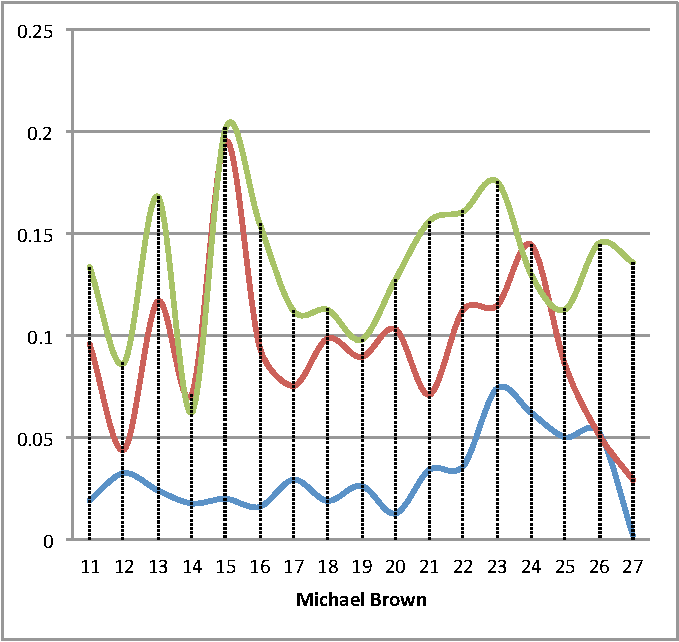
\includegraphics[width=0.22\linewidth]{figures/4_3_Michael_Brown.pdf}
\label{fig:mb}
}
\subfigure[News Report]
{
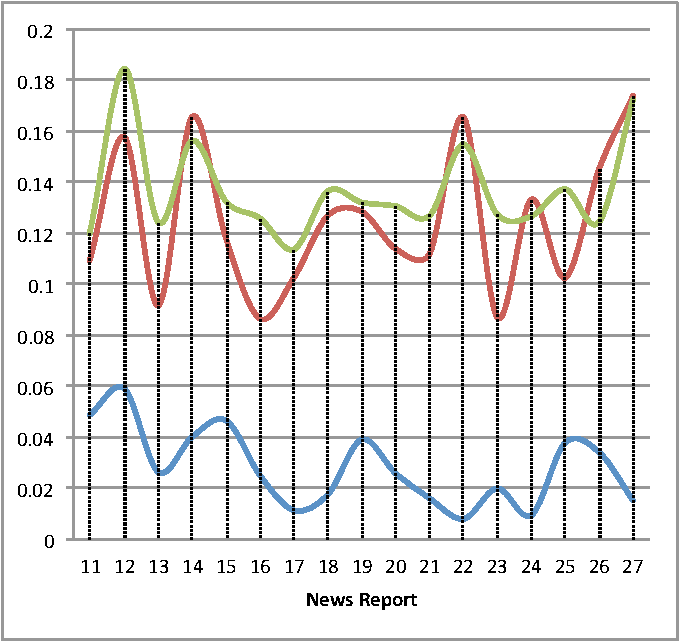
\includegraphics[width=0.22\linewidth]{figures/4_4_News_report.pdf}
\label{fig:news_report}
}
%\subfigure[Racism]
%{
%\includegraphics[width=0.32\linewidth]{figures/4_5_Racism.pdf}
%\label{fig:racism}
%}
\subfigure[Pray]
{
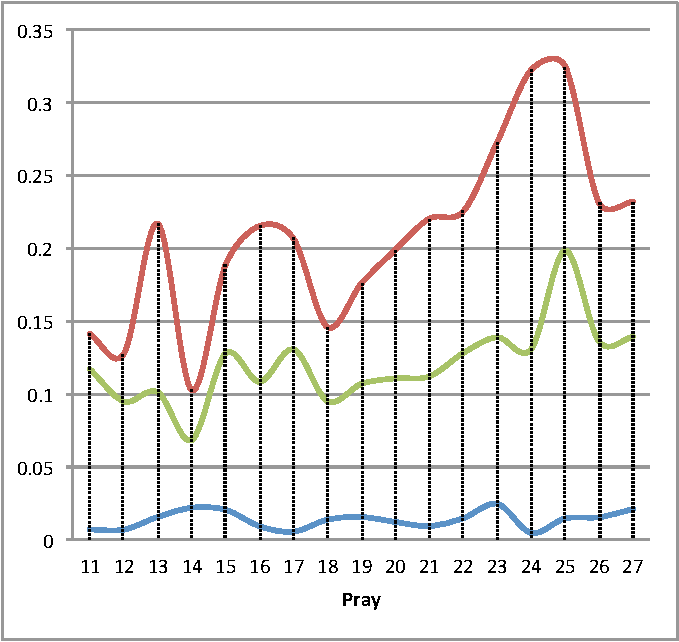
\includegraphics[width=0.22\linewidth]{figures/4_6_Pray.pdf}
\label{fig:pray}
}
\subfigure[Emotion]
{
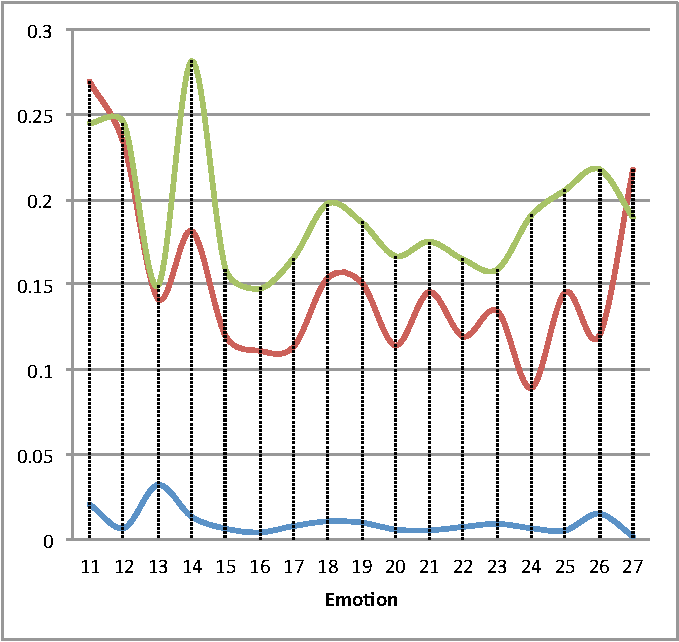
\includegraphics[width=0.22\linewidth]{figures/4_7_Emotion.pdf}
\label{fig:emotion}
}
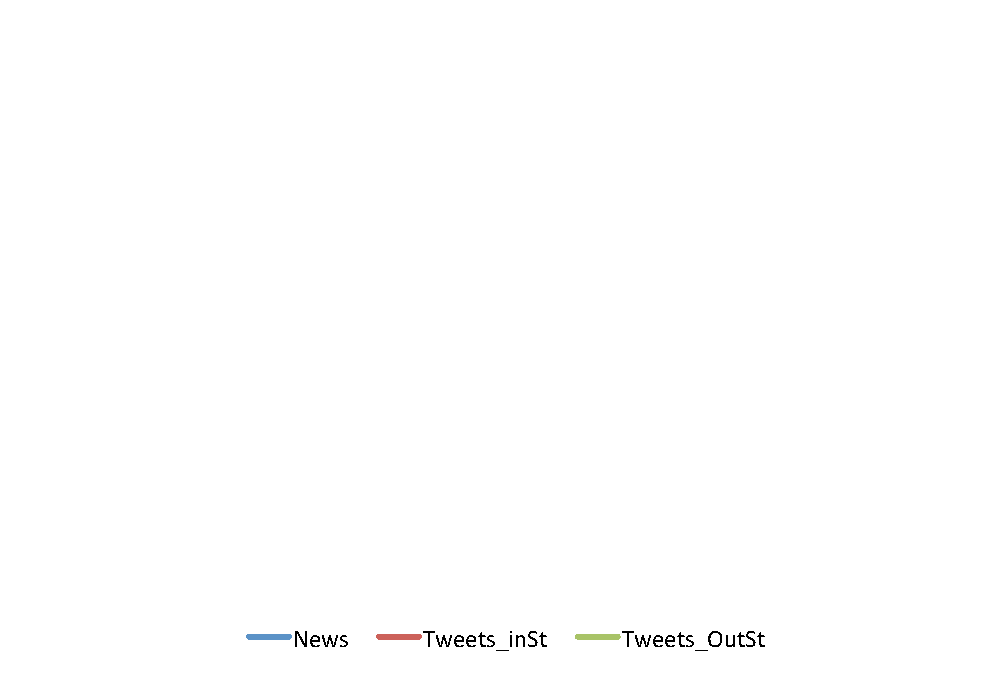
\includegraphics[width=0.5\linewidth]{figures/4_Legend_cut.pdf}
\caption{Topic Dynamic of News and Tweets by \stlda}\label{fig:topics_news_tweets}
\end{figure*}

\subsubsection{Media Influence on the Public}
As Twitter is a self-contained environment, tweets out of \stlouis are also influenced by content in Twitter. So they share similarities with tweets in \stlouis, such as the diversity of topics and similar pattern for topics \pray, \emotion and \newsreport. However analysis of topics also shows that compared to people in \stlouis, their perception of the event relies more on outside source of information rather than self experience, thus they are subjected to be influenced by media more.

Difference between tweets in and out of \stlouis indicates the possible influence from media to the public. Out of \stlouis, the \emotion tweets take the majority on August 12th and 14th, on one day when main media topic is \shootincident, and another day when media increasingly talk about \obamatalk. The rapid growth of \emotion suggests either a long term effect of \shootincident or a quick force of \obamatalk. The two topics are influential, however there is no more fine-grained analysis of what the emotions are, e.g. positive and negative emotions.

\racism is a major topic for tweets out of \stlouis and has an increasing trend, which is consistent with the increasing trend of news talking about \raceandcommunity. The agenda setting of media has actual influence on the public.

In the topic \newsreport, top words such as \emph{news}, \emph{watch}, \emph{live}, \emph{report}, \emph{coverage} and \emph{rt} indicate that the topic is mainly about description or citation of information from news or TV. It is an direct evidence of media influence on tweets. An increase of \newsreport topic tweets means more public attention to news. Interestingly, tweets in and out of \stlouis have similar topic dynamics for \newsreport, meaning that news have similar impact to people both in and out of \stlouis. However, to figure out why the peaks and what news attract public attention, we need more detailed analysis to the reference of news by tweets.

It is also worth noting that proportion of each topic changes more slightly compared to tweets in \stlouis. Although tweets of certain topic may increase in some time, the proportion of tweets in each topic keeps relatively steady. It is possible that people out of \stlouis have different sources of information like news and social media, so their focus is more dispersed under the influence of different information.

\subsubsection{Media Reflection of Public Voices}
In major topics of news, discussion of racism may reflect public concerns, as topic \racism takes an important part of both tweets in and out of \stlouis. It is more likely to be interaction between media and the public with influence in both direction.

Of the minor topics of news, topic \pray and \emotion take a very small part (less than 5\%). It is reasonable that tweets are more subjective and contain more words about feelings, emotions and prays, while news is more serious and objective, avoiding emotional leading. However, even when there is an explosion of \emotion in tweets, or there are increasing tweets talking about \pray, there is no corresponding burst of news topic, which means such emotional change of the public is not reflected in news, or maybe news reacts to the emotions with other topics. However the relation is even harder to detect, because we don't know which news topics are in react to public emotions.
The topic \michaelbrown can be seen as a peak in news followed by increasing tweets of such topic. Then from August 19th increasing tweets in \stlouis start to talk about \michaelbrown again followed by a lag increase pattern of tweets out of \stlouis and news. Except for the funeral of Brown, there are no special events tend to be related to such change. It is possible that when the public pay more and more attention to Michael Brown and the media capture this change and reflect it in news.

In summary, evidence shows the influence of news on tweets, while media reflection of public voices is rare. The existence of \newsreport topic in tweets directly shows the information flow from news to tweets. Comparatively there is no specific topic related to tweets in news. Change of \racism in tweets out of \stlouis may reflect the results of agenda-setting by media. While \emotion change is a possible result by media topics. Because of the media influence, except the main topic \racism, focus of the public is dispersed, while there are different focuses from \emotion, \racism to \protest and \pray along with time for tweets in \stlouis. However, although under the influence of media, tweets do not simply repeat topics of news. Only a small amount of tweets talk about \obamatalk, even though news have steady coverage of \obamatalk during the events. There is no direct evidence showing that news have reflected the opinion changes in tweets. It is possible that news react to tweets topics with other topics, such as the discussion of \raceandcommunity.
